\documentclass[pdflatex,compress]{beamer}

%\usetheme[dark,framenumber,totalframenumber]{ElektroITK}
\usetheme[darktitle,framenumber,totalframenumber]{ElektroITK}
\usepackage{graphicx}
\usepackage{multicol}

\title{Data Communications}
\subtitle{Chapter 5 - Signal Encoding Techniques}

\author{Mifta Nur Farid}

\begin{document}

\maketitle

\begin{frame}
	\frametitle{Encoding and Modulation}
	\begin{center}
		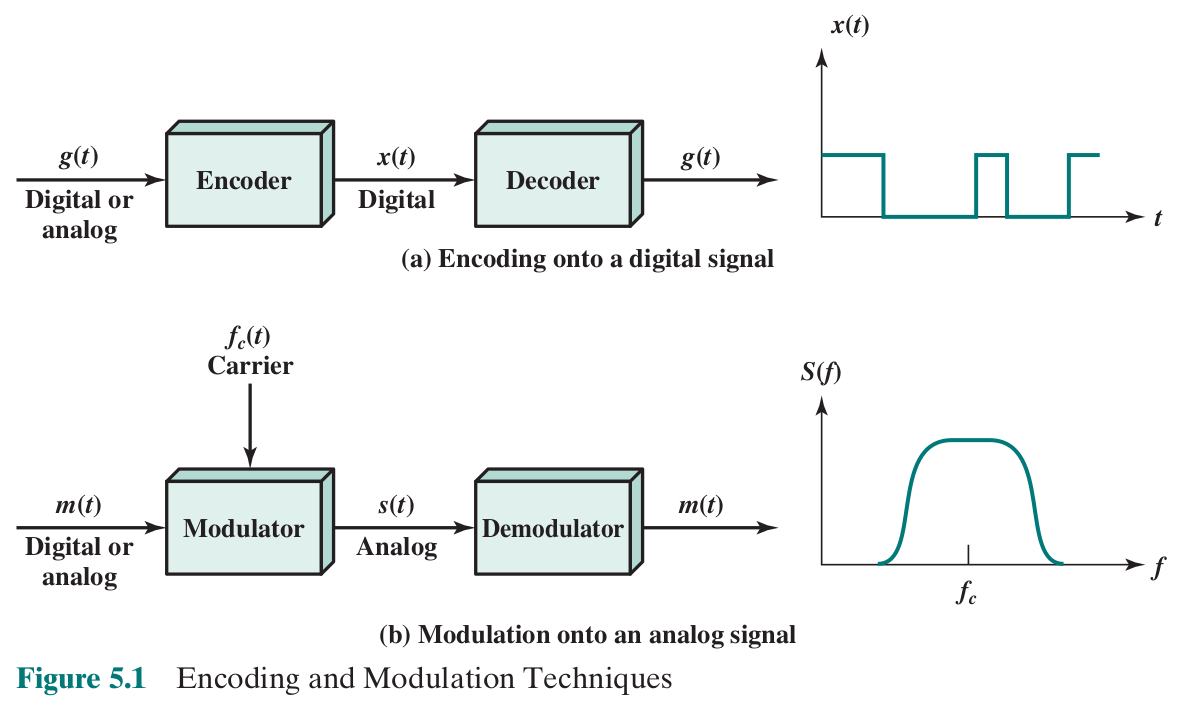
\includegraphics[width=\linewidth]{img/img01}
	\end{center}
\end{frame}

\begin{frame}
	\frametitle{Digital Data, Digital Signal}
	\textbf{Digital signal}
	\begin{itemize}
		\item Sequence of discrete, discontinuous voltage pulses
		\item Each pulse is a signal element
		\item Binary data are transmitted by encoding each data bit into signal elements
	\end{itemize}
\end{frame}

\begin{frame}
	\frametitle{Terminology}
	\begin{itemize}
		\item \textbf{Unipolar}: all signal elements have the same sign
		\item \textbf{Polar}: one logic state represented by positive voltage and the other by negative voltage
		\item \textbf{Data rate}: rate, in bits per second that data are transmitted
		\item \textbf{Duration or length of a bit}: time taken for transmitter to emit the bit
		\item \textbf{Modulation rate}: rate at which the signal level is changed; the rate is expressed in baud, which means signal elements per second
		\item \textbf{Mark and space}: refer to the binary digits 1 and 0
	\end{itemize}
\end{frame}

\begin{frame}
	\frametitle{Key Data Transmission Terms}
	\begin{center}
		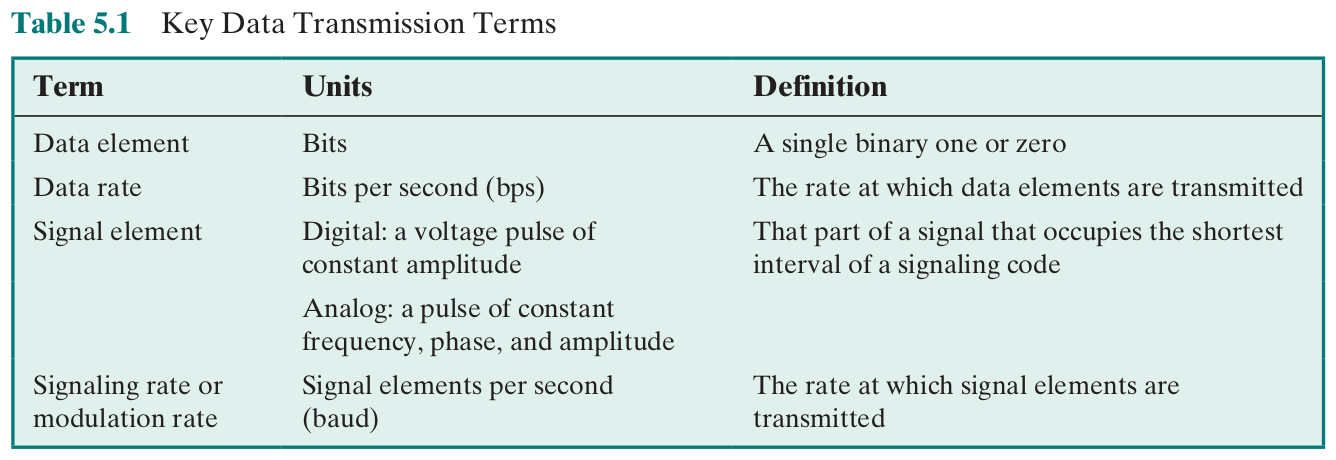
\includegraphics[width=\linewidth]{img/img02}
	\end{center}
\end{frame}

\begin{frame}
	\frametitle{Interpreting Signals}
	\begin{multicols}{2}
		\begin{itemize}
			\centering
			\item[] \textbf{Tasks involved in interpreting digital signal at the receiver:}\\
			\centering $ \downarrow $
			\item[] Timing of bits - when they start and end\\
			\centering $ \downarrow $
			\item[] Signal levels
		\end{itemize}
	\columnbreak
		\begin{itemize}
			\centering
			\item[] \textbf{Factors affecting signal interpretation:}\\
			\centering $ \downarrow $
			\item[] Signal to noise ratio\\
			\centering $ \downarrow $
			\item[] Data rate\\
			\centering $ \downarrow $
			\item[] Bandwidth
		\end{itemize}
	\end{multicols}
\end{frame}
%-----------------------
%  Tugas
%-----------------------

\begin{frame}
	\frametitle{Tugas Mandiri}
	\begin{itemize}
		\item Stallings, W. (2014). Data and Computer Communications, 10th Edition, New Jersey: Upper Saddle River\\
		\begin{itemize}
			\item Chapter 4 Transmission Media
		\end{itemize}
		\item Gupta, P. C. (2006). Data Communications and Computer Networks. New Delhi: Prentice Hall of India\\
		\begin{itemize}
			\item Chapter 2 Transmission Media
		\end{itemize}
		\item Tanenbaum, A. S. \& Wetherall, D. J. (2013). Computer Networks, Fifth Edition. London: Pearson.\\
		\begin{itemize}
			\item Section 2.2 Guided Transmission Media
			\item Section 2.3 Wireless Transmission
			\item Section 2.4 Coammunication Satellites
		\end{itemize}
	\end{itemize}
\end{frame}

\begin{frame}
	\frametitle{Tugas Terstruktur}
	\textbf{Tampilkan Tugas 3}
\end{frame}

\end{document}
